\section{Association Analysis} \label{association analysis}

Association rule mining is the task of finding associations between \textit{items} in a database of \textit{transactions}. The technique was originally developed in 1993 to identify patterns in consumers grocery purchasing behaviour~\cite{Agrawal:1993:MAR:170036.170072}. Since then however, association analysis has found applications in wide variety of domains.

Association rule mining is an attractive method for modelling non-linear relationships of variables. Many of the mobile device system settings and context variables are highly dependent on one another and therefore their combined effect on the energy consumption is difficult to estimate using linear models. Many non-linear modelling techniques require additional knowledge about the structure of the data. Association rule mining requires relatively few assumptions about the data to be made. In fact the only preprocessing that is necessary in order to apply the association rule mining, is data discretization.    

Let us consider a hypothetical dataset shown in table~\ref{table:raw-data}. The dataset consists of mobile device system settings and energy usage measurements. The dataset has three continuous valued variables:  energyRate, the rate at which the battery is discharging;  CPULevel, the device's CPU usage level and screenBrightness, the brightness of the device's screen. Each of these variables takes floating point values ranging from 0.0 to 1.0.
\begin{table}[b] %[htb]
	\centering
    \begin{tabular}{ | l | l | l | }
    \hline
    \textbf{energyRate} & \textbf{CPULevel} & \textbf{screenBrightness} \\ \hline
    0.21 & 0.58 & 0.30 \\ \hline 
    0.80 & 0.46 & 0.61 \\ \hline 
    0.76 & 0.65 & 0.93 \\ \hline 
    0.58 & 0.99 & 0.54 \\ \hline 
    \end{tabular}
	\caption{Hypothetical mobile device measurements inspired by Carat dataset}
	\label{table:raw-data}
\end{table}

Since association rule mining requires each variable of the database to be binary valued, a discretization of the variables must be performed. To discretize a continuously valued variable, we need to replace the continuous variable with multiple binary valued variables, each corresponding to an interval or cluster of values of the continuous variable. The details of discretization of Carat data are discussed in Chapter~\ref{carat data}. For simplicity, let us consider a simple discretization strategy, where each continuous variable is split to two binary variables by creating two bins at cut point 0.5. Tables \ref{table:discreteData-1} and \ref{table:discreteData-2} demonstrate this idea.

%\begin{table}[htb]
%    \begin{tabular}{ | l | l | l | l | l | l | }
%    \hline
%    \textbf{energy=low} & \textbf{energy=high} & \textbf{CPU=low} & \textbf{CPU=high} & \textbf{screen=low} & \textbf{screen=high} \\ \hline
%    True & False & False & True & True & False \\ \hline 
%    False & True & True & False & False & True \\ \hline 
%    False & True & False & True & False & True \\ \hline 
%    False & True & False & True & False & True \\ \hline 
%    \end{tabular}
%	\caption{Hypothetical mobile device measurements after naive discretization}
%	\label{table:discreteData}
%\end{table}

\begin{table} %[htb]
	\centering
    \begin{tabular}{ | l | l | l | }
    \hline
    \textbf{energy=low} & \textbf{energy=high} & \textbf{CPU=low} \\ \hline
    True & False & False  \\ \hline 
    False & True & True  \\ \hline 
    False & True & False  \\ \hline 
    False & True & False  \\ \hline
    \end{tabular}
	\caption{Hypothetical mobile device measurements after discretization using long notation. First half of the columns.}
	\label{table:discreteData-1}
\end{table}

\begin{table} %[htb]
	\centering
    \begin{tabular}{ | l | l | l | }
    \hline
    \textbf{CPU=high} & \textbf{screen=low} & \textbf{screen=high} \\ \hline
	True & True & False \\ \hline
	False & False & True \\ \hline    
    True & False & True \\ \hline
    True & False & True \\ \hline
    \end{tabular}
	\caption{Hypothetical mobile device measurements after discretization using long notation. Second half of the columns.}
	\label{table:discreteData-2}
\end{table}


Since every group of variables that is created by discretization is mutually exclusive, a more concise notation for this dataset can be used, as shown in Table~\ref{table:discreteDataConcise}.

\begin{table} %[htb]
	\centering
    \begin{tabular}{ | l | l | l |}
    \hline
	\textbf{energyRate} & \textbf{CPULevel} & \textbf{screenBrightness} \\ \hline
    low & high & low  \\ \hline 
    high & low & high \\ \hline 
    high & high & high \\ \hline 
    high & high & high \\ \hline 
    \end{tabular}
    \caption{Hypothetical mobile device measurements after discretization using concise notation}
    \label{table:discreteDataConcise}
\end{table} 

%As an example, consider a hypothetical database of following transactions denoting individual mobile device system settings, extracted from the Carat data:
 
%\begin{center}
%    \begin{tabular}{ | l | l | }
%    \hline
%    \textbf{Items} \\ \hline
%    cpuLevel=high, energyRate=high \\ \hline 
%    diapers, beer, cookies \\ \hline 
%    diapers, beer, bread \\ \hline 
%    butter, bread, cheese \\ \hline 
%    \end{tabular}
%\end{center} 
 
%The goal of the association analysis is then to produce a list of association rules, given a some measure of interestingness. From the database given above, some algorithm might produce the following association rules: 

Having transformed the raw data to binary variables, the goal of the association analysis is then to produce a list of association rules, given some measure of interestingness. For the database given above, an association rule mining algorithm might find the following association rule 

\[
	\left\{ CPULevel=high, screenBrightness=high \right\} \Rightarrow \left\{ energyRate=high \right\}
\]

This rule implies that high CPU utilization together with high screen brightness associates with high level of energy consumption.

\subsection{Formal Problem Definition}

Let $I = \left\{ x_1, x_2, ..., x_n \right\}$ be a set of binary variables called items. A transaction database $T$ is then a multiset of subsets of $I$, where each element of $T$ denotes a transaction. To give the exact problem of association rule discovery, concepts of support and confidence need to be introduced.

Support of an item set $X$ in database $T$ is defined as the fraction of all transactions in $T$ that contain the item set~\cite{Hipp:2000:AAR:360402.360421}.

\[ supp(X) = \dfrac{ \vert \left\{ X' \in T  \mid X \subseteq X'  \right\}  \vert }{ \vert T \vert  } \]

Confidence of a rule $X \Rightarrow Y$, where $X$ and $Y$ are item sets of $T$, is defined as the fraction of transactions in $T$ containing item set $X$ which also contain $Y$~\cite{Hipp:2000:AAR:360402.360421}.

\[conf( X \Rightarrow Y) = \dfrac{ supp( X \bigcup Y ) }{ supp(X) } \]

The problem of association rule discovery can now be formalized the following way. Given a transaction database $T$, minimum support level $s$, where $ 0 \leq s \leq 1 $ and minimum confidence level $c$, where $ 0 \leq c \leq 1 $, find all rules $X \Rightarrow Y$ where $conf( X \Rightarrow Y ) \geq c$, $supp(X) \geq s$ and $supp(Y) \geq s$~\cite{Hipp:2000:AAR:360402.360421}. 

The association rule discovery problem can be further divided into two distinct sub-problems, namely frequent pattern mining problem and rule generation problem. A frequent pattern $P$ of database $T$ is a subset of $I$ such that $supp(P) \geq s$. The frequent pattern mining problem is the task of finding all frequent patterns from a given database. The rule generation problem on the other hand, is the task of generating all association rules with sufficient confidence from the frequent patterns. 

%\subsection{Frequent Pattern Mining Using Frequent Pattern Growth}
\subsection[Frequent Pattern Mining Using Frequent Pattern Growth]{Frequent Pattern Mining Using Frequent\\ Pattern Growth}

Frequent pattern growth is an efficient algorithm for the frequent pattern mining problem~\cite{Han:2000:MFP:335191.335372}. The FP-growth algorithm has been shown to outperform the time consumption of traditional Apriori pattern mining algorithm~\cite{Agrawal94fastalgorithms} by more than an order of magnitude when mining large databases~\cite{Han:2000:MFP:335191.335372}. The algorithm utilizes a specialized data structure called FP-tree, a kind of prefix tree, to speed up the frequent pattern generation. The FP-tree data structure consists of nodes, each of which have tree fields: item name, item count and node link. The item name tells which item the node represents. The item count signifies the number of transactions containing the item, that can be reached by following the path of nodes in the FP-tree leading to this node. The node link contains a pointer to the next node in the FP-tree with the same node name. An exception to this format is the root node of the FP-tree, which does not have any of these fields, but only has links to child nodes. Algorithm~\ref{Algorithm:FP-tree} shows how to constructs a FP-tree for a transaction database~\cite{Han:2000:MFP:335191.335372}.

\begin{algorithm}[!htbp]
	\SetAlgoLined\DontPrintSemicolon
	\SetKwFunction{buildFPTree}{buildFPTree}\SetKwFunction{insertTree}{insertTree}
	\KwData{A transaction database \textit{DB}, minimum support threshold \textit{s}}
	\KwResult{FP-tree for the database}
	\SetKwProg{myalg}{Algorithm}{}{}
	\myalg{\buildFPTree{\textit{DB}, \textit{s}}}{
		\nl	\textit{F} $\leftarrow$ Scan \textit{DB} and collect a map of items and their frequencies\;
		\nl \textit{L} $\leftarrow$ Sort keys of \textit{F} in descending order of support filtering out items which have support < \textit{s}\;
		\nl \textit{T} $\leftarrow$ root node of the FP-tree\;
		\nl \For{ transaction \textit{Trans} \textbf{in} \textit{DB} }{ 
			\nl sort \textit{Trans} according to \textit{L} and filter out infrequent items\;
			\nl insertTree(\textit{Trans}, \textit{T})\;
		}
		\nl \KwRet{\textit{T}}\;
	}
	\setcounter{AlgoLine}{0}
	\SetKwProg{myproc}{Procedure}{}{}
  	\myproc{\insertTree{\textit{Trans}, \textit{T}}}{
		\nl \If{\textit{Trans} is empty}{
			\nl \KwRet\;
		} \nl \Else{
			\nl	\textit{N} $\leftarrow$ first item of \textit{Trans}\;
			\nl \textit{tail} $\leftarrow$ tail of \textit{Trans}\;	
			\nl \If{ \textit{T} has a child \textit{h} such that \textit{N}.item-name == \textit{h}.item-name} {
				\nl \textit{h}.count += 1\;
				\nl insertTree(\textit{tail}, \textit{h})
			} \nl \Else {
				\nl \textit{n} $\leftarrow$ create new node with item-name = \textit{p}.item-name and count = 1 and link \textit{T} as its parent\;
				\nl insertTree(\textit{tail}, \textit{n})
			}
		}
	}	
	\caption{Fp-tree construction}
	\label{Algorithm:FP-tree}
\end{algorithm}  

The algorithm consists of two procedures. The entry point for the algorithm is the \textit{buildFPTree}-procedure, which takes no parameters and returns the newly built FP-tree. The sub-program \textit{insertTree} takes a transaction \textit{Trans}, that is sorted by descending item frequency, and an incomplete FP-tree \textit{T} as its parameters. The \textit{insertTree} procedure walks down \textit{T} in a path determined by the items in \textit{Trans}, incrementing the counts of nodes on the path. If there is no existing path to walk down on at any point, the \textit{insertTree} creates a new node with count 1 as a child of the last node that was walked over.

The \textit{buildFPTree} procedure proceeds the following way. In line 1, the transaction database is scanned and the different item names together with their frequencies are collected to variable \textit{F}. In line 2, keys of \textit{F} are sorted in descending order of support and items which have support less than minimum support \textit{s}. The sorted and filtered key-count-pairs are stored in variable \textit{L}. In line 3, the root of node of the FP-tree is created and stored in variable \textit{T}. In line 4, a for loop that iterates over each transaction in the transaction database is entered. The loop yields the transactions in a variable called \textit{Trans}. In line 5, the contents of variable \textit{Trans} are sorted according to the ordering induced by \textit{L} and infrequent items (items which have support that is less than \textit{s}) are filtered out of \textit{Trans}. In line 6, the sub-program \textit{insertTree} is called passing parameters \textit{Trans} and \textit{T}. The for loop entered on line 4 is exited. Finally on line 7, \textit{T}, which now contains the complete FP-tree, is returned.  

The \textit{insertTree} procedure consists of the following steps. In lines 1-3, we check if parameter \textit{Trans} is empty and return if so. In lines 4-5, we store the first item of parameter \textit{Trans} in variable \textit{N} and the rest of the items in variable \textit{tail}. In line 6, we enter an if statement with the conditional "\textit{T} has a child \textit{h} such that \textit{h} has the same item name as \textit{N}". In line 7 we increment the count of \textit{N} by one. In line 8 we call \textit{insertTree} recursively with parameters \textit{tail} and \textit{h}. In line 9, we exit the then-branch of the if statement and enter the else-branch. In line 10, we create a new node with item-name equal to \textit{N}, count equal to 1 and we link \textit{T} as the node's parent. The newly created node is stored in variable \textit{n}. In line 11 we call \textit{insertTree} recursively with \textit{tail} and \textit{n} as its parameters.

To better illustrate the process of building an FP-tree from a transaction database, let us go through an example that uses a simple made up transaction database. First step of building a FP-tree, is to sort each transaction by decreasing order of frequency of its items in the database. Infrequent items are also filtered out based on the minimum support. Table~\ref{table:fp-growth-example1} shows the example transaction database as well as the frequent items in descending order of frequency. A single traversal over the database is required in order to sort the transactions.

For this example, let us consider a minimum support of 0.3. Since the number of transactions in our database is 6 and $ \frac{1}{6} < 0.3 < \frac{2}{6} $, all items with frequency less than 2 can be filtered out. Thus items i and j are not included in the second column of table~\ref{table:fp-growth-example1}. 

\begin{table} %[!htbp]
\begin{center}
    \begin{tabular}{ | l | l | }
    \hline
	\textbf{Items} & \textbf{Frequency Ordered and Filtered Items} \\ \hline
    a, b, c, d, e, h & c, e, h, a, b, d \\ \hline 
    c, d, e, h & c, e, h, d \\ \hline 
    c, e, h & c, e, h \\ \hline 
    a, b, c, e, j & c, e, a, b \\ \hline 
    c, h & c, h \\ \hline
    d, i & d \\ \hline
    \end{tabular}
    \caption{Example transaction database for illustrating FP-tree generation.}
    \label{table:fp-growth-example1}
\end{center}
\end{table} 

To construct the FP-tree we start with a node labelled as "root". We then take the first transaction and walk over its elements in the frequency order. We start from the root node of the FP-tree. Since the roo node has no child nodes, we add a child node labelled with "c" and set its count to 1. We remove the item "c" from the transaction being handled. Then we continue the walk from the node labelled with "c". The procedure is repeated with the remaining items of the transaction, continuing the walk from the node labelled "c". The FP-tree after processing the first transaction is shown in Figure~\ref{figure:fp-growth-example1}.

\begin{figure} %[!htbp]
	\centering
	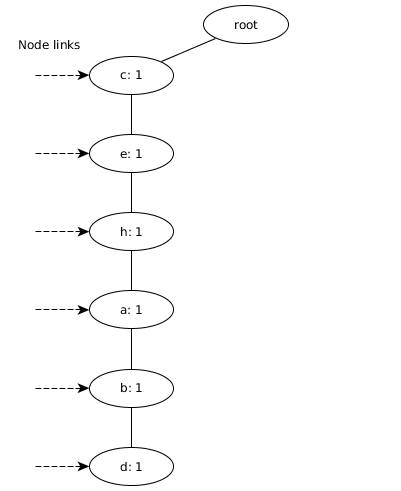
\includegraphics[scale=0.5]{fp-tree-example/fp-tree-p1.png}
	\caption{FP-tree after processing the first transaction}
	\label{figure:fp-growth-example1}
\end{figure}

Next, the second transaction is processed as follows. We again start walking down FP-tree from the root node processing items in the second transaction. Since the root node has a child node labelled with "c" we increment its count to 2 and remove item "c" from the transaction being processed. Since the node has a child node labelled with "e" and our next item to be processed is "e", we move to the node labelled with "e" and increment its count by one and remove item "e" from the transaction being processed. The same process is applied to item "h" and the node labelled with "h". The next item to process is "d", but the node labelled with "h" does not have a child node labelled with "d". We therefore add a child node labelled with "d" and add 1 to the count of the node labelled with "h". Figure~\ref{figure:fp-growth-example2} shows the progress after processing the second transaction of the database.

\begin{figure} %[!htbp]
	\centering
	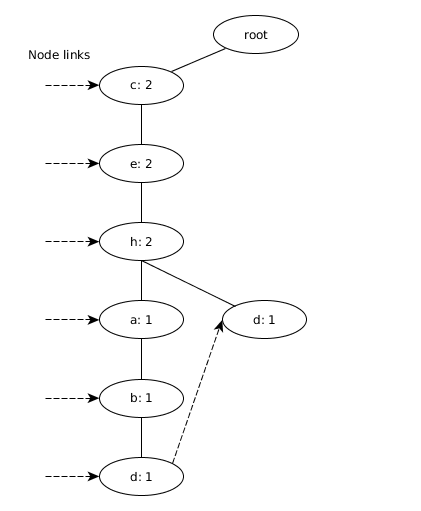
\includegraphics[scale=0.5]{fp-tree-example/fp-tree-p2.png}
	\caption{FP-tree after processing the second transaction}
	\label{figure:fp-growth-example2}
\end{figure}

Repeating the same procedure for the rest of the transactions yields complete FP-tree as illustrated in Figure~\ref{figure:fp-growth-example3}.

\begin{figure} %[!htbp]
	\centering
	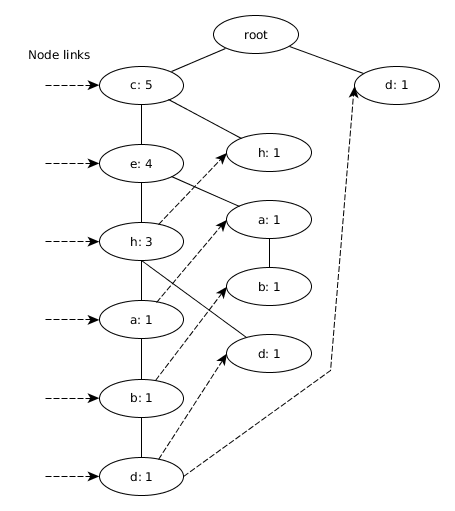
\includegraphics[scale=0.5]{fp-tree-example/fp-tree-p3.png}
	\caption{Complete FP-tree}
	\label{figure:fp-growth-example3}
\end{figure}

The dashed arrows in Figure~\ref{figure:fp-growth-example3} represent node links. The FP-tree maintains a table of linked lists for each distinctly named item. Whenever a node is added to the FP-tree, a pointer to that node is also added to the linked list corresponding to that nodes label.

\begin{figure} %[!htbp]
	\centering
	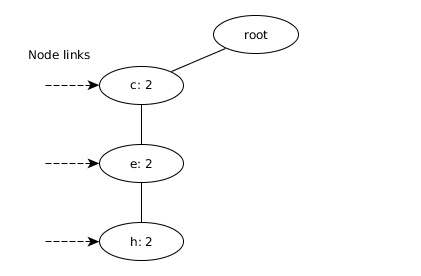
\includegraphics[scale=0.5]{fp-tree-example/fp-tree-conditional.png}
	\caption{Conditional FP-tree of item d.}
	\label{figure:fp-tree-conditional}
\end{figure}


The way an FP-tree is constructed guarantees, that all FP-trees have the so called \textit{node-link property}~\cite{Hipp:2000:AAR:360402.360421}. What it means, is that for any frequent item, all frequent patterns containing that item can be constructed by following the item's node-links starting from the item's head in the FP-tree header. Let us consider the FP-tree in Figure~\ref{figure:fp-growth-example3}. Starting from the bottom of the node links, we examine which frequent patterns can be extracted by following the node link. For item "d", we can trivially extract a frequent pattern "d:3". In addition, we have to consider the three prefix paths of "d" which are accessible from the node links of item "d": (c:5, e:4, h:3, a:1, b:1, d:1), (c:5, e:4, h:3, d:1) and (d:1). These three paths form the \textit{conditional pattern base}~\cite{Hipp:2000:AAR:360402.360421} of "d". To extract all frequent patterns containing item "d", we start by substituting all the item counts in each of the prefix paths in the conditional pattern base of "d" with the count of "d" in the prefix path. This is done to account for the fact that on each of the prefix paths of "d", the other items appear together with "d" exactly as many times as "d" itself. We also leave out the element "d" itself. We now get the transformed conditional pattern base (c:1, e:1, h:1, a:1, b:1), (c:1, e:1, h:1). The next step towards the frequent patterns containing "d", is to construct a \textit{conditional FP-tree} of "d"~\cite{Hipp:2000:AAR:360402.360421}. The construction of the conditional FP-tree conforms to the same set of rules as a normal FP-tree. The only difference is that a prefix path in the conditional pattern base, such as (x:n, y:n, z:n) should be interpreted as \textit{n} distinct transactions containing the items x, y and z. Figure~\ref{figure:fp-tree-conditional} shows the conditional FP-tree of item d constructed from the transformed conditional pattern base. Since there is only a single path in the conditional FP-tree, one can generate all the remaining frequent patterns containing item d by taking all combinations of items c, e, h and concatenating them with d. Each such pattern has support equal to the minimum support among the items in the combination. In this case, we would get frequent patterns \{cd:2, ed:2, hd:2, ced:2, chd:2, ehd:2, cehd:2\} in addition to the trivial pattern d:3. But what would happen if the conditional FP-tree contained multiple paths? In this case one would recursively construct a new conditional FP-tree for the item whose node link yields multiple paths. Following this procedure for each node link in the original FP-tree, one can generate all the frequent patterns.  

\begin{algorithm}[!htbp]
\SetAlgoLined\DontPrintSemicolon
	\SetKwFunction{FPGrowth}{FPGrowth}\SetKwFunction{patternGrowth}{patternGrowth}
	\KwData{\textit{FP-tree} constructed using Algorithm~\ref{Algorithm:FP-tree}, minimum support threshold \textit{s}}
	\KwResult{All frequent patterns of the database}
	\SetKwProg{myalg}{Algorithm}{}{}
	\myalg{\FPGrowth{\textit{FP-tree}, \textit{s}}}{
		\nl	patternGrowth(\textit{FP-tree}, \textit{null})
	}
	\setcounter{AlgoLine}{0}
	\SetKwProg{myproc}{Procedure}{}{}
  	\myproc{\patternGrowth{\textit{tree}, \textit{sub-pattern}}}{
		\nl \If{\textit{tree} contains only single path \textit{P}}{
			\nl \For{ each combination \textit{C} of items in \textit{P}}{ 
				\nl generate frequent pattern $\textit{C} \cup \textit{sub-pattern}$ with support = minimum support of items in \textit{C} \;
			}
		} \nl \Else{
				\nl \For{ each node in the header of \textit{tree} }{ 
					\nl \textit{C}  $\leftarrow$ pattern $\textit{node.item} \cup \textit{sub-pattern}$ with support = \textit{node}.support  \;
					\nl generate pattern \textit{C} with support = \textit{node}.support \;
					\nl \textit{B} $\leftarrow$ construct conditional pattern base of \textit{C} constrained by minimum support threshold \textit{s} \;
					\nl \textit{T} $\leftarrow$ construct the conditional FP-tree of \textit{C} from \textit{B} constrained by minimum support threshold \textit{s} \;
					\nl \If{\textit{T} is non-empty}{
						\nl patternGrowth(\textit{T}, \textit{C}) \;
					}
				}
			}
	}	
	\caption{Fp-growth}
	\label{Algorithm:FP-growth}
\end{algorithm}

Formalizing the method discussed above yields Algorithm~\ref{Algorithm:FP-growth}~\cite{Hipp:2000:AAR:360402.360421}. The algorithm \textit{FPGrowth} takes as its arguments an FP-tree and a minimum support threshold. In line 1 of the algorithm, a procedure \textit{patternGrowth} is called with the FP-tree and an empty sub-pattern denoted by value \textit{null}. The procedure \textit{patternGrowth} has two parameters. The first parameter is a conditional FP-tree and the second parameter is the sub-pattern for which the conditional FP-tree was built. Initially, the procedure will be called with the whole FP-tree and empty sub-pattern. The algorithm will recursively simplify the conditional FP-tree until the tree only contains a single branch, from which the frequent patterns can be easily generated. In line 1, the procedure checks if the conditional FP-tree only has one branch. If so, the frequent patterns of the conditional FP-tree are outputted in lines 2-3 after which the procedure is finished. If the conditional FP-tree had more than one branch, we go to line 5, where we start to iterate over all nodes reachable from the conditional FP-tree's header's node-links. In line 6, we create a new pattern by appending the node's item to the current sub-pattern. The pattern is stored to variable \textit{C}. The new pattern's support is set to be equal to the support of the node that is being iterated. In line 7, the pattern \textit{C} is appended to the output of the program. In lines 8-9, a conditional FP-tree of pattern \textit{C} is constructed and stored in variable \textit{T}. In lines 10-11 we recursively call \textit{patternGrowth} with the newly constructed conditional FP-tree \textit{T} and pattern \textit{C}. After line 11, we exit the iteration loop and the procedure is finished.           

\subsection{Generating Association Rules from Frequent Patterns}

The frequent patterns may reveal some interesting structures in the transaction database, as they effectively capture frequent co-occurrence of various items. Although this may be enough for some application domains, it is often the case that one would ultimately want to reveal some causal relationships between items or sets of items in the database. The association rules offer a rudimentary but fairly scalable solution for discovering "if X then Y" type of relationships between subsets of items in the frequent patterns. It should be noted here, that the field of causal inference expands far beyond scope of this thesis work and the association rules should at best be considered as candidates for causal relationships, not as proofs of such.

Given a set of frequent patterns \textit{F}, and a minimum confidence threshold \textit{c}, the task of generating the association rules can be accomplished by the following method: 
%Iterate through each set of items \textit{I} in \textit{F}. Iterate over each non-empty subset \textit{A} of \textit{I}. If $conf(A \Rightarrow I \setminus A ) \geq \textit{c}$ then output rule $A \Rightarrow I \setminus A$.

\begin{enumerate}
	\item For each set of items \textit{I} in \textit{F}
	\begin{enumerate}
		\item For each non-empty subset \textit{A} of \textit{I}
		\begin{enumerate}
			\item If $conf(A \Rightarrow I \setminus A ) \geq \textit{c}$ then output rule $A \Rightarrow I \setminus A$
		\end{enumerate}
	\end{enumerate}
\end{enumerate}      

While the proposed method does work when the size of the frequent patterns is small, this approach quickly becomes infeasible as the length of the patterns grow. Given a frequent pattern \textit{I} with $\mid\textit{I}\mid$ items, there are a total of $2^{\mid\textit{I}\mid}$ subsets of which $2^{\mid\textit{I}\mid} - 2$ need to be tested as the set \textit{I} itself and the empty set can be discounted. Fortunately, a technique exists for pruning the search space, as described by Agrawal et al.~\cite{Agrawal:1994:FAM:645920.672836}. The confidence measure has the anti-monotone property, meaning that for any frequent pattern $I = \{A, B, C, D\}$ the following inequality holds:

\[ conf(ABC \Rightarrow D) \geq conf(AB \Rightarrow CD) \geq conf(A \Rightarrow BCD) \] 

\begin{algorithm}[!htbp]
\SetAlgoLined\DontPrintSemicolon
	\SetKwFunction{generateRules}{generateRules}
	\KwData{A set of frequent patterns \textit{F}, a minimum confidence threshold \textit{c}}
	\KwResult{Association rules discovered from the frequent patterns}
	\SetKwProg{myalg}{Algorithm}{}{}
	\myalg{\generateRules{\textit{F}, \textit{c}}}{
		\nl \For{each frequent pattern \textit{P} in \textit{F}}{ 
			\nl \textit{C} $\leftarrow$ candidate rule generator of \textit{P} ordered by increasing length of candidate rule's consequent set length \;
			\nl \While{\textit{C} has more candidate rules}{ 
				\nl \textit{r} $\leftarrow$ get next candidate rule from \textit{C} \;
				\nl \If{ $conf(\textit{r}) \geq \textit{c}$ }{
					\nl output \textit{r} \;
				}
				\nl \Else{
					\nl Remove all candidates rules \textit{r'} from \textit{C} where $r.consequents \subset r'.consequents$ \;
				}
			}		
		}
	}	
	\caption{Generating association rules from frequent patterns}
	\label{Algorithm:generate-association-rules}
\end{algorithm}

Since moving items from the antecedent set to the consequent set never increases the confidence of the rule, one can potentially prune an enormous amount of candidate rules by iterating the candidate rules in ascending order of length of the candidate rule's consequent set~\cite{Agrawal:1994:FAM:645920.672836}. After each iteration, if the candidate rule being processed did not have high enough confidence, then all remaining candidate rules whose consequent set contains a subset of the current candidate rules consequent set, can be pruned since the anti-monotone property guarantees that any such rule has confidence no higher than the current candidate rule. 

Algorithm~\ref{Algorithm:generate-association-rules} gives an outline on how to generate association rules from frequent patterns with search tree pruning. The details of how to generate the combinations of items and how to implement the pruning of the search space are not presented here. The algorithm takes a set of frequent patterns and a minimum confidence threshold as its arguments and returns the set of association rules discovered from the frequent patterns. In line 1 we start to iterate over the frequent patterns. In line 2 we initialize the candidate rule generator storing it to variable \textit{C}. In line 3, we enter a while loop which is terminated when generator \textit{C} has no more candidate rules to generate. In line 4 we store the next candidate rule from \textit{C} to variable \textit{r}. In lines 5-6, we test if the confidence of candidate rule \textit{r} is greater or equal to the minimum confidence threshold and output the rule if the criteria is met. If the confidence criteria was not met, we prune the candidate rule space of generator \textit{C} in lines 7-8.        